\documentclass{beamer}
\usepackage[utf8]{inputenc}
\usetheme{Madrid}
\usecolortheme{default}

% math & fonts
\usepackage{amsmath,amssymb,amsthm}
\usepackage{txfonts}
\usepackage{lmodern}

% drawing / figures / listings
\usepackage{tkz-euclide}
\usepackage{tikz}
\usepackage{graphicx}
\usepackage{listings}
\usepackage{xcolor}
\usepackage{array}
\usepackage{tabularx}
\usepackage{adjustbox}

% (optional) your local package; comment if not available
\usepackage{gvv}

% vector macro
\newcommand{\myvec}[1]{\begin{bmatrix}#1\end{bmatrix}}

% show total frame count in footer
\setbeamertemplate{page number in head/foot}[totalframenumber]

% listing defaults
\lstset{
    language=C,
    basicstyle=\ttfamily\small,
    keywordstyle=\color{blue},
    stringstyle=\color{orange},
    commentstyle=\color{green!60!black},
    numbers=left,
    numberstyle=\tiny\color{gray},
    breaklines=true,
    showstringspaces=false,
}

\title{Matgeo-q.4.13.1}
\author{AI25BTECH11036-SNEHAMRUDULA}
\date{\today}

\begin{document}

\begin{frame}
  \titlepage
\end{frame}

\section{Question}
\begin{frame}{Question}
Consider the lines
\[
\begin{aligned}
L_1 &: x + 3y - 5 = 0, \\
L_2 &: 3x - ky - 1 = 0, \\
L_3 &: 5x + 2y - 12 = 0.
\end{aligned}
\]
Match the statements in Column I with Column II (choices refer to values of \(k\) or relations).
\begin{center}
\begin{tabular}{p{0.45\linewidth} p{0.45\linewidth}}
\textbf{Column I} & \textbf{Column II} \\
\begin{enumerate}[label=(\Alph*)]
    \item $L_1, L_2, L_3$ are concurrent, if
    \item One of $L_1, L_2, L_3$ is parallel to at least one of the other two, if
    \item $L_1, L_2, L_3$ form a triangle, if
    \item $L_1, L_2, L_3$ do not form a triangle, if
\end{enumerate}
&
\begin{enumerate}[label=(\alph*)]
    \item $k = 9$
    \item $k = \dfrac{-6}{5}$
    \item $k = \dfrac{5}{6}$
    \item $k = 5$
\end{enumerate}
\end{tabular}
\end{center}
\end{frame}

\section{Solution}
The three line equations can be written in matrix form as
\begin{align}
    \myvec{
    1 & 3 \\
    3 & -k \\
    5 & 2
    }\vec{x}
    =
    \myvec{5\\1\\12}.                                   \label{eq:mainmatrix}
\end{align}

\textbf{(A) Concurrency}
The lines are concurrent when all three equations admit a common solution.  
This happens if
\begin{align}
    \rank\myvec{1 & 3 \\ 3 & -k \\ 5 & 2}
    =
    \rank\myvec{1 & 3 & 5 \\ 3 & -k & 1 \\ 5 & 2 & 12}
    = 2.                                               \label{eq:concurrency}
\end{align}
Expanding the augmented determinant condition gives
\begin{align}
    k &= 5.                                            \label{eq:kconcurrent}
\end{align}

\textbf{(B) Parallelism}
Two lines are parallel when their normals are proportional.  
Equivalently, $\rank$ of the normals is $1$:
\begin{align}
    \rank\myvec{\vec{n}_2 & \vec{n}_3} = 1.            \label{eq:parallelrank}
\end{align}
This gives
\begin{align}
    k &= -\tfrac{6}{5}.                                \label{eq:kparallel}
\end{align}

\textbf{(C) Triangle condition}
Three lines form a triangle if they intersect pairwise but are not concurrent.  
That is,
\begin{align}
    \rank\myvec{\vec{n}_1 & \vec{n}_2} 
    = \rank\myvec{\vec{n}_2 & \vec{n}_3} 
    = \rank\myvec{\vec{n}_3 & \vec{n}_1} = 2, \quad
    k \neq 5,\; k \neq -\tfrac{6}{5}.                  \label{eq:trianglecond}
\end{align}
So among the given options,
\begin{align}
    k = 9 \quad \text{or} \quad k = \tfrac{5}{6}.      \label{eq:ktriangle}
\end{align}

\textbf{(D) Do not form a triangle}
This occurs if either concurrent or parallel, i.e.
\begin{align}
    k = 5 \quad \text{or} \quad k = -\tfrac{6}{5}.     \label{eq:notriangle}
\end{align}
\begin{align}
    (A)&\to (d): k=5, \\
    (B)&\to (b): k=-\tfrac{6}{5}, \\
    (C)&\to (a)\;\text{or}\;(c): k=9 \;\text{or}\;\tfrac{5}{6}, \\
    (D)&\to (d)\;\text{or}\;(b): k=5 \;\text{or}\; -\tfrac{6}{5}.
\end{align}

\begin{frame}{Graphical Representation}
\begin{center}
% placeholder figure drawn with TikZ
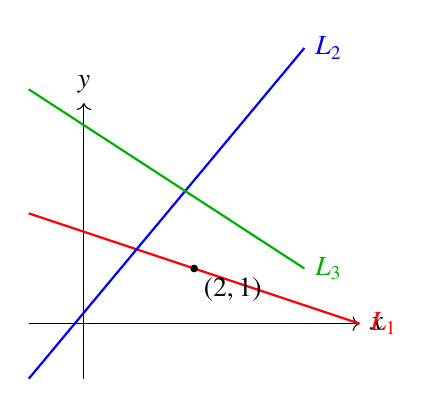
\begin{tikzpicture}[scale=0.7]
  % Axes
  \draw[->] (-1,0)--(5,0) node[right]{$x$};
  \draw[->] (0,-1)--(0,4) node[above]{$y$};

  % Lines
  \draw[red, thick] (-1,2) -- (5,0.0) node[right] {$L_1$};
  \draw[blue, thick] (-1,-1) -- (4,5) node[right] {$L_2$};
  \draw[green!70!black, thick] (-1,4.25) -- (4,1) node[right] {$L_3$};

  % Intersection point
  \fill (2,1) circle (2pt) node[below right] {$(2,1)$};
\end{tikzpicture}
\end{center}
\end{frame}

\end{document}
